\documentclass[onecolumn, draftclsnofoot,10pt, compsoc]{article}
\usepackage{graphicx}
\usepackage{url}
\usepackage{lscape}
\usepackage{setspace}
\usepackage{parskip}
\usepackage{geometry}
\usepackage{listings}
\geometry{textheight=9.5in, textwidth=7in}

% 1. Fill in these details
\def \CapstoneTeamName{AgBizClimate}
\def \CapstoneTeamNumber{26}
\def \GroupMemberOne{	Thomas Noelcke}
\def \GroupMemberTwo{	Shane Barrantes}
\def \GroupMemberThree{	Shengpei Yuan}
\def \CapstoneProjectName{ Linking Seasonal Weather Data to AgBizClimate\texttrademark}
\def \CapstoneSponsorCompany{ Oregon State University}
\def \CapstoneSponsorPerson{ Clark Seavert}

% 2. Uncomment the appropriate line below so that the document type works
\def \DocType{		%Software Requirements Document
				%Requirements Document
				%Technology Review
				%Design Document
				Mid Term Progress Report Winter 2018
				}

\newcommand{\NameSigPair}[1]{\par
\makebox[2.75in][r]{#1} \hfil 	\makebox[3.25in]{\makebox[2.25in]{\hrulefill} \hfill		\makebox[.75in]{\hrulefill}}
\par\vspace{-12pt} \textit{\tiny\noindent
\makebox[2.75in]{} \hfil		\makebox[3.25in]{\makebox[2.25in][r]{Signature} \hfill	\makebox[.75in][r]{Date}}}}
% 3. If the document is not to be signed, uncomment the RENEWcommand below
\renewcommand{\NameSigPair}[1]{#1}

%%%%%%%%%%%%%%%%%%%%%%%%%%%%%%%%%%%%%%%
\begin{document}
\begin{titlepage}
    \pagenumbering{gobble}
    \begin{singlespace}
        \hfill
        % 4. If you have a logo, use this includegraphics command to put it on the coversheet.
        %\includegraphics[height=4cm]{CompanyLogo}
        \par\vspace{.2in}
        \centering
        \scshape{
            \huge CS Capstone \DocType \par
            {\large\today}\par
            \vspace{.5in}
            \textbf{\Huge\CapstoneProjectName}\par
            \vfill
            {\large Prepared for}\par
            \Huge \CapstoneSponsorCompany\par
            \vspace{5pt}
            {\Large\NameSigPair{\CapstoneSponsorPerson}\par}
            {\large Prepared by }\par
            Group\CapstoneTeamNumber\par
            % 5. comment out the line below this one if you do not wish to name your team
            %\CapstoneTeamName\par
            \vspace{5pt}
            {\Large
                \NameSigPair{\GroupMemberOne}\par
                \NameSigPair{\GroupMemberTwo}\par
                \NameSigPair{\GroupMemberThree}\par
            }
            \vspace{20pt}
        }
        \begin{abstract}
					 The purpose of this document is to give a snap shot of the current state of the project. In this progress report will start off by discussing ToDo's we have resolved. We will then move on to items that are in progress. After that we will discuss what is still left to do on the project. Next we will give a week by week summary of our progress including our plans for each week, what we accomplished, problems we encountered and a summery for the week. Finally, In the last section of this report we will each talk about our individual contributions to the project along with a peer review for each of our group mates.\\
        \end{abstract}
    \end{singlespace}
\end{titlepage}
\newpage
\pagenumbering{arabic}
\tableofcontents
% 7. uncomment this (if applicable). Consider adding a page break.
%\listoffigures 
\newpage
%\listoftables
\clearpage

% 8. now you write!
%this section can likely be coppied from the design doc.
\section{Introduction}
	\subsection{Purpose}
		The purpose of this document is to describe the progress we have made so far on the \textit{AgBizClimate} project. In this document we will give a brief introduction to the \textit{AgBizCliamte} project. In this section we will discuss the purpose of the project. Additionally, we will also discuss the scope of the project and an overview of the project functions.\\
		This document is designed for the project owners. This document is also designed for the development team so we can evaluate our progress so far on this project. This project is also designed to fulfill the minimum requirements for the CS461 class for the OSU computer science program.\\

				\subsection{Overview}
			Seasonal climate is one of the essential factors that affects agricultural production. As a module of \textit{AgBiz Logic}, \textit{AgBizClimate} delivers essential information about climate change to farmers, and help professionals to develop management pathways that best fit their operations under a changing climate. This project aims to link the crucial seasonal climate data from the Northwest Climate Toolbox database to \textit{AgBiz Logic} so that it can provide changes in net returns of crop and livestock enterprises through powerful graphics and tables.\\

		\subsection{Scope}
			This project is a part of a much larger AgBiz Logic\texttrademark program. However, the purpose of this project is to add a short term climate tool to the \textit{AgBizClimate} module. This limits the scope of the project to the \textit{AgBizClimate} Module. Additionally, we will only be adding the short term climate data tool as the long term climate data tool already exists.\\

			Currently \textit{AgBizClimate} has a long-term climate tool but no such tool exists for short term climate data. We will implement a tool to extract short-term climate data from the Northwest Climate Toolbox database, display it to the user and allow the user to adjust crop and livestock yields or quality of products sold and, production inputs. Moreover, a landing tool will be developed to allow users to switch between short-term seasonal tool and long-term climate data tool.\\

		\subsection{Definitions, Acronyms and Abbreviations}
			REST - Representational State Transfer, This is a type of architecture that manages the state of the program. This is especially popular in web development.\\
			API- Application Programming Interface. This is a piece of software that allows a connection to another piece of software providing some sort of service.\\
			NWCTB - Northwest Climate Toolbox. This is the database we will be connecting to that will provide the short term climate data we plan to use.\\
			Thredds Data Server - This is a web server that provides meta-data and data access for scientific data sets using OPeNDAP along with some other remote data access protocols.\\
			OPeNDAP - Open-source Project for a Network Data Access Protocol. This is the protocol we will be using to retrieve the data sets from the Thredds data server.\\
			NMME - North American Multi-Model Ensemble. This is a data set that brings together a variety of different weather models into one data set.\\
			Climate Scenario - This is a theoretical calculation of yields, inputs and of the overall budget for one situation based on the climate data.\\
			NETCDF - This is a file storage format for large scientific data sets especially good for any data that is referenced on a grid and related to is geo-location.\\


		%will need updates.
		\subsection{Product Function Overview}
		    \textit{AgBizClimate} is a web based decision tool that will allow users to gain specific insight on how localized climate data for the next seven months will affect their crop and livestock yields or quality of products sold and production inputs. The \textit{AgBizClimate} tool will allow users to input their location (state, county) and a budget for the specific crop or livestock enterprise. \textit{AgBizClimate} will select climate data for the next seven months for that location and provide graphical data showing temperature and precipitation. Users will then be able to change yields or quality of product sold by a percentage they think these factors will affect and modify production inputs. Finally the tool will calculate the net returns.\\



		\renewcommand\refname{\vskip -1cm}
		\subsection{References}

		    \nocite{*}
            \bibliographystyle{IEEEtran}
            \bibliography{IEEEabrv,References}


\section{Current Project State}
    In this section of this document we will review what items we have resolved, List and explain what items we still have to do, discuss major blockers and give a week by week summary of what we have done so far. This section is intended to give a good overall picture of the status of the \textit{AgBizClimate} project along with what we have accomplished so far.\\

	\subsection{Resolved Items}
		\paragraph{Updated Requirements Document:} The requirements document has been updated to reflect changes to the climate data API. We were expecting to have an endpoint we could call with a latitude and a longitude however accessing the climate data is going to require more work that we had originally expected. So we've updated the requirements document to reflect this change.\\


		\paragraph{Create Concept script for Thredds database:} We've created a concept script to use as an example in our climate API that connects to the Thredds database and read back the climate data for the Latitude and Longitude we've request. However, we are getting errors on reads latter in the data set that we can't explain.\\


		\paragraph{Install Script for NETCDF4 and Dependencies:} Another problem we encountered while creating the concept script was setting up and installing the python NETCDF4 library. Luckily we were able to write a scrip that installs this library and its dependencies.\\

		\paragraph{Added option to select Short term Climate Scenario:} We added a drop down to the region selection page that allows users to select short term climate scenarios and long term climate Scenarios. This will allow people to use the tool we are creating.\\

		%this isn't actually true yet but I'm working on it and getting close.
		\paragraph{Created The Charts Page:} We've also created the page where the users will view the climate data. This page will also allow the users to enter a change in yield for their crops and will then redirect them to the Budget review page. Though this page has a few issues most of the work is completed.\\


	\subsection{In progress}
	In this section we will discuss work items that are in active development. We will describe each item giving a brief description. We will also discuss how much progress has been made on each item.\\

		\paragraph{Climate Data API:} We have started work on the back end Climate data API however currently it is just an end point that distributes mocked data as we have run into issues with the netcdf4 library we are using to connect to the database with all the data in it. Once we have a solution for connecting to and reading all the values from the database it won't be hard to get real data from the API.\\

		\paragraph{Document Updates:} We have had some serious changes to the expected design as a result we will need to make some document updates. We have started some of these updates. However, I don't anticipate being able to finish all the document updates this term.\\

	\subsection{ToDo's}
	    In this section we will discuss items we will need still need to do over the next two terms. We will give a brief description of each item. We will also state an approximate time for when we expect each item to be completed.\\

			\paragraph{Backend Testing:} Given that our Climate data has not yet been well defined we haven't started writing test to test the back end code. Once we get the API written in something close to its final form we will want to start writing some test to ensure that the API meets the requirements in the requirements document.\\

			\paragraph{Front End testing:} Similarly as the front end work is still in active development we haven’t written any tests to cover this code. However we will be done with front end development soon and should be able to get to work doing front end testing.\\

			\paragraph{Finding a solution to NETCDF4 Problems:} We will need to find a work around to get around errors we are having while reading from the database using the netcdf4 library. Currently, we think we can get around this by writing the bit that communicates with the server in c++. However we are trying installing dependencies for the netcdf library in a different way first.\\

			\paragraph{QA:} Finally, before we are done with our project will want to provide some QA on the work that we will have done over the term. This will include running some manual integration tests to ensure that we have completed the work we agreed to complete.\\

	\subsection{Blockers}
	    In this section we will discuss hurtles we are facing that are impeding progress on this project. We will discuss why they will keep us from moving forward on this project and we will also discuss what we intend to do to move past these problems.\\

			\subsubsection{netcdf problems}
			Initially, we had issues getting netcdf4, a python library for dealing with the data files that contain the

	%will copy from one note. Will need to modify weekly summary from each week just a tiny bit to make this section work
\section{Weekly summary of progress}
	   In this section we will give a weekly summary of our progress on this project. For each we will list out our plans, problems we have encountered during the week and will show a summery of what we have accomplished during the week.\\

		\subsection{Week 1}
			\subsubsection{Plans}
				\begin{itemize}
					\item Meet with group to set up iteration one of project development.
					\item Meet with Sean to set up git branch and discuss git workflow.
					\item set taks for iteration 1.
				\end{itemize}

			\subsubsection{Progress}
				\begin{itemize}
					\item Forked github repo from AgBiz-Logic
					\item Set up a meeting with Sean to discuss project development.
					\item Started setting up tasks for iteration one on the git repo.
					\item Started working on the Wiki page with common help items for the project.
				\end{itemize}
			\subsubsection{Problems}
				\begin{itemize}
					\item Still haven't heard any thing from the NWCTB team regarding API access for the climate data.
				\end{itemize}

			\subsubsection{Summary}
			This week we tried to set up a meeting with Sean to do some project planning and set up for iteration one of our project. However, Sean was unavailable this week so we set up a meeting for next week. We also got our git repo, forked from \textit{AgBiz-Logic} set up. We started planning the first iteration of development on the project by adding issues to the github repository. We also started compiling some help pages on the Wiki of our repo.\\

		\subsection{Week 2}
			\subsubsection{Plans}
				\begin{itemize}
					\item Meet with Sean.
					\item Start Iteration One.
					\item Get UI elements implemented along with most of the front end functionality.
					\item Plan iterations 2 and 3.
				\end{itemize}
			\subsubsection{Progress}
				\begin{itemize}
					\item Set up meeting with Sean Hammond for Friday at 1 pm.
					\item Finished setting up iteration one tasks.
					\item Finished adding content to the help wiki on the github repository.
					\item Finally defined Climate Data API Access.
					\item Set a Weekly status meeting time to meet with the group. We plan to meet every week at one pm.
				\end{itemize}
			\subsubsection{Problems}
				\begin{itemize}
					\item API Access is less than ideal and will require more work than we were planning on but is still better than having to write our own service from scratch.
					\item Finding time to meet up as a group has been more challenging that I had anticipated.
				\end{itemize}

			\subsubsection{Summary}
			This week we didn't get much development work done on our project like we had planed on. However, we did do some set up work. we finished setting up the github repository and finished laying out tasks on our story board. We also started defining what tasks we'd like to have in future iterations of our project. Additionally, we finally know what our API access to the climate data looks like. this will allow us to get the data we will need to plot. However, this will also require much more work that we had planned on and may set us back a bit in terms of our project schedule. That being said we worked in some flex time in to our schedule so we should be able to make it work.\\

		\subsection{Week 3}
			\subsubsection{Plans}
				\begin{itemize}
					\item Create proof of concept script for connecting to the database and getting data.
					\item start working on front end changes.
					\item Update design document and requirement document.
					\item Meet with Sean for status update at 1pm on Friday.
				\end{itemize}
			\subsubsection{Progress}
				\begin{itemize}
					\item Started working on concept script.
					\item Managed to gt dev environment set up instructions completed.
					\item Installed netcdf.
					\item Created example script for getting climate data from the thredds database. However we get some errors on certain reads.
					\item Updated requirements document.
				\end{itemize}
			\subsubsection{Problems}
				\begin{itemize}
					\item We had a hard time getting NETCDF4 to install. We ended up using anaconda however we are guessing Sean doesn't want to use Anaconda and will want us to produce an install script.\\
				\end{itemize}
			\subsubsection{Summary}
			This week was a primarily a week of setup. we spent most of our time trying to get the dev environment set up along with installing NETCDF4 and its dependencies. This week we did find a way to install NETCDF4 using anaconda. However, we anticipate that we will be required to find a better way to install it. In the mean time this will allow us to develop a concept script. We also managed to the development environment for AgBiz-Logic set up. This took us more time that we had anticipated but wasn't as difficult as we thought it might be. This week we also made some updates to the requirements document to reflect the changes to the climate data API.\\

		\subsection{week 4}
			\subsubsection{Plans}
				\begin{itemize}
					\item Start working on the front end of the application.
					\item Refine the proof of concept to be more dynamic.
					\item Write script to install netcdf and dependencies.
					\item Start working on backend changes.
					\item Update documents.
				\end{itemize}
			\subsubsection{Progress}
				\begin{itemize}
					\item Started working on refining proof of concept script to search for points if the point we asked for doesn't have data also added more advanced bounds checking.
					\item Determined that NETCDF4 is having issues reading in blocks for chunk three.
				\end{itemize}
			\subsubsection{Problems}
				\begin{itemize}
					\item requests past index 435 on latitude cause a runtime error.
				\end{itemize}
			\subsubsection{Summary}
			This week was mostly focused on working on the proof of concept scrip that will be used later to access the data from the thredds server. This week we discovered that the NETCDF4 library throws errors on any lat index greater than 435. We also discovered through the database administrator that this is the boundary between chunk two and chunk three of the file we are trying to read. We think that the NETCDF4 library may have a bug in it. Regardless we are going to need to find a work around moving forward. Shane and Thomas also got together on Saturday and started working on front end changes.\\

		\subsection{week 5}
			\subsubsection{Plans}
				\begin{itemize}
					\item Work on front end changes.
					\item Follow up with NETCDF4 developers about potential bug.
					\item Continue to work on concept script to see if we can tease out the runtime error.
					\item Finish NETCDF5 install script.
					\item Research other potential options other than python or netcdf4 for reading in data from the serer.\\

				\end{itemize}
			\subsubsection{Progress}
				\begin{itemize}
					\item Followed up with netcdf4 people.
					\item Shane finished the netcdf4 install script.
					\item Researched alternatives to netcdf4 We can write a c program that will to the same thing. There are a few other libraries for reading data via opendap.
					\item made progress on frontend changes.
				\end{itemize}

			\subsubsection{Problems}
				\begin{itemize}
					\item Issues with netcdf4 library.
					\item netcdf4 developers will not fix unless I can produce a self contained example of the read failing.
					\item We think that netcdf4 dependencies may not be installed correctly.
				\end{itemize}

			\subsubsection{Summary}
			 This week we made progress on the front end development and installing the dependencies for netcdf. However, we've run into some issues with netcdf. We think we maybe able to fix it by installing the dependencies for netcdf from source with certain flags enabled but we aren't totally sure on that. We also started work on setting up the end point where the API will live. The plan for now is to have it serve mock data as to enable us to continue with the rest of the development work without getting behind.\\

		%will fill out this section later this week.
		\subsection{week 6}
			\subsubsection{Plans}
				\begin{itemize}
					\item Finish development of the charts page.
					\item Set up API to mock data.
					\item Figure out work around for netCDF problems.
					\item write the midterm progress report.
					\item make the midterm progress presentation.
					\item finish the poster rough draft.
				\end{itemize}
			\subsubsection{Progress}
				\begin{itemize}
					\item Finished Development on the charts page.
					\item Finished the midterm progress report.
					\item Made the midterm progress report presentation.
					\item Finished the Poster rough draft.
					\item Found a work around for NETCDF4 issues.
				\end{itemize}
			\subsubsection{Problems}
				\begin{itemize}
					\item Created some bugs by introducing short term climate scenarios.
						\subitem There are many ways we can fix this problem we will need to discuss with Sean how he wants this solved.
				\end{itemize}
			\subsubsection{Summary} This week was a busy week. This week we accomplished most of the front end development required by this project in the maps page. However, we also introduced some bugs. Mostly we created and issue where if you have multiple budgets its not possible to tell what page you need to redirect to once you save your budget. There are many ways we can solve this so I want to ask Sean how he thinks the best way to go about this is. This week we also made our expo poster along with creating the midterm progress report document and presentation. Additionally, Shengpei found a work around to the NETCDF problems we've been having.\\


\section{Individual Section}
In this section we will each write about our individual parts of the project and the progress we have made. We will also use this section to provide a peer review for our group mates rating their performance and contribution to the project.\\

\subsection{Thomas Noelcke}
	In this section I will discuss the various contributions I've made to the project along with some of the problems I've come across including any solutions to problems that I’ve found. I will also discuss the contribution of my team mates to this project giving each of my group mates a peer review.\\

	\subsubsection{My Contributions}
		Through out this project I've had the opportunity to work on many aspects of the project. So far I've worked on the concept script, documentation, and worked on the front end. However, these are not my sections below in the section titled My Sections I will explain why what I've wored on so far does not relate to my sections in the technical review.\\

		\paragraph{Concept API Script} \hfill \break
		One of the fist things I worked on this term was creating a concept script that connected with the Thredds sever and read in NETCDF climate data from the the server. We decided to use netcdf4 over the OPeNDAP protocol because this was what the database administrator suggested we use. The goal of this script was to prove that it was possible to use the NETCDF4 library and python to retrieve the data we needed for our project. In the end the script I worked on proved to be a dead end. Though through the process of writing this script I learned a lot about how scientific data storage works. Its actually really unfortunate that the netcdf4 library didn't work out for us. This frame work was really easy to use and nice to work with. Essentially with this frame work we were able to treat the database like a giant array. Shown below is some code that demonstrates this capability.\\

\begin{lstlisting}
#set up the data handles to filter the data
filehandle = Dataset(path, 'r', format="netcdf3")
lathandle = filehandle.variables['lat']
lonhandle = filehandle.variables['lon']
datahandle = filehandle.variables['prate_anom']

#gets data from the server.
print(datahandle[466, 1083, 0])
\end{lstlisting}
		
In the end this library threw errors when trying to read in chucked data from the server. I ended up spending a few days trying to debug this issue. It resulted in the netcdf4 developers stating they wouldn't look into this issue unless we could produce a self contained example of this failure. Ultimately Shengpei ended up finding another solution to this problem with out using the NETCDF library so I passed the development of the concept script off to him.\\

		\paragraph{Documentation} \hfill \break
		Another item I worked on this term was updating the requirements document as a result of changes to the climate API. I made modifications to the glossary and to the functional requirements to reflect the changes made to the project. The big change made to the project was a change in the API Access. This necessitated the updating of the requirements of the project. These changes reflect the fact that we have to to more work than we expected to retrieve the climate data.\\


		\paragraph{Front-end Work} \hfill \break
		The other section of the application that I've spent a lot of my time on this term is front end development. The first change that I made was to the region selection page. On this page I added a drop down that allows the user to select between a long term climate scenario and a short term climate scenario. This drop down then posted back to the database and also redirects the flow of the application based on the scenario the user selects. If the user selects a long term scenario they are redirected to a page that allows them to select different variables that effect long term climate projections. If the user selects a short term climate Scenario they are redirected to the chart page where they are shown the climate data.\\
		
		The other section of the front end development that I have been working on is the Charts page. This page charts four different climate plots over the next 7 months. This then allows the user to switch to the different charts using a tab system. This page also allows the user to enter a percent change in their yield that will then be applied to their budget. Once they enter a yield they will then be redirected to a budget page where they can review their budget and make adjustment to inputs and costs for the various inputs. Shown below is a screen shot of this page.\\
		
		\clearpage
		\newpage
		\begin{figure}[h!]
		\centering
		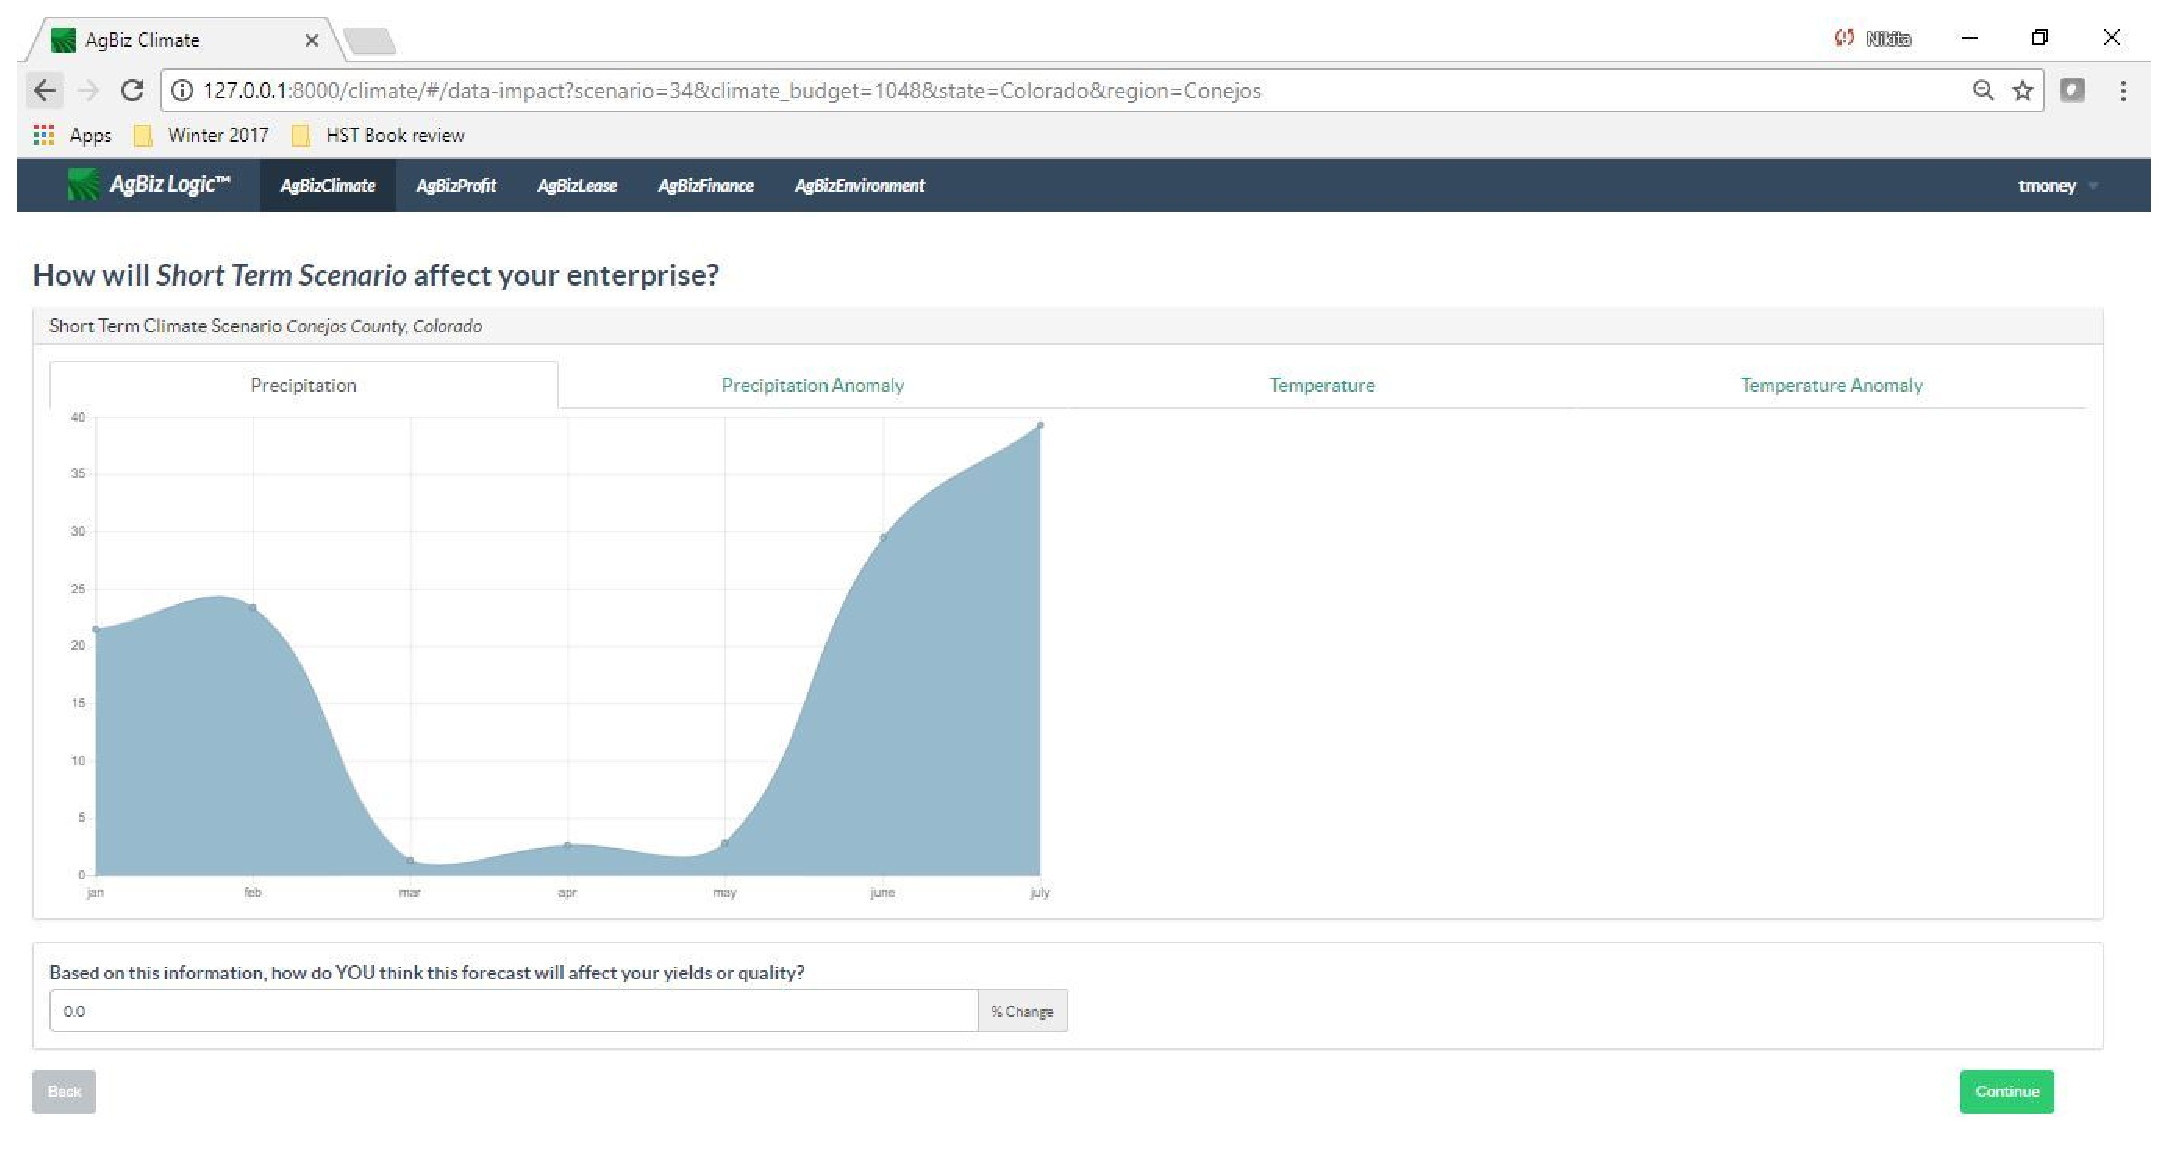
\includegraphics[width=17cm]{chartsPage.eps}
		\caption{Charts Page}
		\end{figure}
		
As you can see from the graph above in created a box that holds the charts and a box that holds the yields. I chose to do the because for a long term Scenario you would enter a change in yield for each climate factor that you would like to consider. For instance if you consider Temperature and nights below freezing you would add a percent change in yield for each of these projections. However, for a short term scenario you are shown four graphs. To reduce confusion I moved the percent yield input box into its own box on the web page so that it would be clear to the user that they are only entering one percent yield for all four charts. Though this graphs page will get the job done I anticipate that as we start working on our stretch goals the charts page will require more work. This is because we would like to add more models to the graph. Another stretch goal that will require modifications to the charts page is adding a confidence interval to our chart. This will require us to use more advanced features of the chart JS library.\\ 

 		\paragraph{My Sections} \hfill \break
		In the tech review my sections were the database, the testing frameworks and the HTTP frame work. I have only spend minimal time working on these sections because there just isn't that much work as relates to this project in these sections. I have not written many unit test yet because we have not developed that much testable code yet. I also haven’t spent any time working on the database because we've not made any data changes requiring migrations just yet. I have however spend some time working on with our HTTP framework while making request to the back end from the front end while doing front end development. As this project progresses I expect that I will be required to make some changes to the database as we make changes to the back end. I also anticipate that we will be required to write many different unit test as we get closer to finishing this project. In fact I expect that I will be writing unit test for the front end soon as we are nearly done with our front end development.\\


\subsection{Shane Barrantes}
	\subsubsection{Goals}
        The primary goal of our team is to implement a system inside the AgBizClimate module that allows farmers and ranchers to view short term climate data (7 months out) for a specified location in the United States and use an AgBizLogic decision algorithm that alters their budgets based how they think the climate will affect their crops or livestock. In short, we want to make a decision tool that assists farmers and ranchers by saving them money based on local short term climate data and their professional experience. It's important to note that in the creation of this portion of AgBizClimate we are maintaining consistent use of technology to the other components of the AgBizClimate module as well as the greater AgBiz-Logic suite of tools.
        \subsubsection{Progress}
	The AgBizClimate team has made substantial progress on the overall completion of our project despite varying roadblocks that have slowed us down along the way. We currently have almost all front end changes implemented, except for unit tests and debugging. We also have also attempted several different ways of pulling data from the Northwest Climate toolbox and have just finished a functional method to get the data via the URL. Now we just need to spend some time on the back end to make it receive and serve that climate data dynamically, add unit tests, update our formal documentation, and attempt to accomplish our stretch goals before the term is over.
	\subsubsection{Contributions}
	In this section I will be discussing the portions of the project that I have primarily been working on over the course of the last six weeks. These portions include team environment setup, build scripts, front-end development, and debugging.
	\paragraph{team environment setup}
        When we began working on the AgBizClimate project we found that their internal documentation looked excellent and quite up to date. However, their build instructions for environment setup were quite convoluted and a bit overkill for what we were trying to do. To combat this and make life easier for the other members of my team I created a new set of build instructions which included links and commands to make the dependencies build on the OSX and Ubuntu operating systems with minimal effort. This allowed us to circumvent clunky VM technologies such as Rocket and Vagrant that would have been a hassle to setup, add great cost to the startup times, and were completely unnecessary to our development life cycle. Basically when something went wrong with somebodies environment, or our build process did not make sense I took it upon myself to fix and better it.
        \paragraph{Build Scripts}
	Early on in the project we found that in order to access data from the Northwest Climate toolbox we had to use NetCDF with OPeNDAP support. This represented a blockade for us because dependencies were quite difficult to find and build. So I built a basic build script for my teammates to use to surmount this issue and to make their lives easier. Eventually we found that the base install of NetCDF would not fulfill our needs so I figured out how to build each component from source with the correct flags and paths. Unfortunately, this too failed so we began looking at the underlying C library for NetCDF instead of the Python overlay, but after tinkering and research we decided this was not the correct avenue for us to be taking and moved on to more promising and expedient solutions which my other group members will give more insight into.
        \paragraph{Front-End Development}
        Initially when front-end development began Thomas and I split the two primary pages between us. I began development on the meaty "charts" page and he added a drop down bar to the location page. However, due to problems with our data gathering pipeline which was used to access the climate data and get it into our web application in a timely matter, I quickly moved away from the front-end development part of the project in an attempt to surmount the other issues we were having. Thomas then took over primary responsibility for the front-end including the charts page so my impact in this space so far has been quite small. I expect that once we have a working data gathering pipeline I will move back to this space in the second half of the term.
        \paragraph{Debugging}
        During the first iteration of our Python script to hit the Northwest Climate API I spent time assisting Thomas in the debugging and logical implementation of our pipeline. We were having a persistent issue when trying to run the script from his local machine where the data would cause an out of bounds error when accessing certain viable locations based on latitude and longitude. After testing this script on both of our machines, plenty of research, and a closed Github issue we chose to pursue other solutions to save time and make things easier.
        \paragraph{My Sections} 
        The three sections I was assigned during the technology review we submitted last term were front-end frameworks, back-end frameworks, and graphing-frameworks. Over the duration of our progress our group found that these technology choices were made for us or had little to do with the actual implementation for our project. Due to this we have been shuffling the tasks between group members based on personal expertise or to assist when one group member may be stuck. This has been nice as it really makes the group feel like a team as we all have similar goals and different takes on the problems. To be more specific the front-end framework we are using is the AngularJS framework which was mandatory based on client specification since they wanted a homogeneous environment. The back-end framework is technically MVC, however we are also implementing a rest API endpoint so that users can access the climate data. Finally the graphing framework Angular-chartJS, was also required by client specification and has played a mostly minor part in the progress so far.


\subsection{Shengpei Yuan}
		\paragraph{Briefly recaps the project purposes and goals} \hfill \break
		The project is dedicated to call essential climate data from a professional climate toolbox database and deliver them in various ways to agriculture producers and land managers in order to help them develop better crop plans and achieve better harvest. Generally, the project contains two key tasks to accomplish the final goal. First, appropriate climate forecast database has to be chosen so that the system could call desired climate data in various ways according to the application contexts. Secondly, the immediately collected climate data should be appropriately stored and presented to users with different demands. In particular, the system would offer comprehensive data APIs for AgBizClimate web programs to extract and demonstrate interested climate data including the changing trends.\\
		It is clear that we would mainly employ the Python program language and the powerful Django web framework to finish the project. And we adopt the popular MVC (Model-View-Controller) design pattern for the overall system architecture. During the past one term, I have finished some substantial work for the project. First, I have reviewed three candidate web design techniques for the project including containers, back end models and frameworks, and styling frameworks. Although I have little practical experiences on some of the web development tools or models, I did roughly learn their general application scenarios and advantages and disadvantages over each other, which may be quite useful for my future studies or work in the area of web design. Second, I have drafted and revised the controller design that is an important part of the overall design document. As an interface between Model and View, the controller plays an important rule in the in the Django MVC idea of the system architecture.\\

		\paragraph{The parts currently working on and the left work to do} \hfill \break
		As a member of the energetic team for the project, it is currently my responsibility to define and implement the climate data API. More specifically, the system could call the API to get climate forecast data back from some authoritative and professional climate database in a flexible form. In addition, it would be expected that the API could be set up like a service on the back end and called directly by any programs at any time when it is necessary. Also it is one of my partners work to transform the workable climate data API scripts into the Django app. \\
		With regards to the future tasks, I would also focus on the backend climate data API. During the entire term of development of the project, the detailed requirements of API may change in some ways. Also the parameters such as model and climate variables need to be considered thoroughly when design the API interfaces. Last but not least important, it is necessary to write both unit and integration tests to ensure that each single function code and the entire system works exactly the same as we have expected in most scenarios.\\
		Action items for the project currently include the Python program scripts for proof of conceptual design of API that call climate data from remote climate databases and updated documents of the project.\\

		\paragraph{The troublesome problems and relevant solutions} \hfill \break
		There are several troublesome problems we may have or need to solve to make the climate forecast data API work correctly. \\
		First, how to call or retrieve climate data of one point that are concerned from the website URL providing downscaled climate forecast data without downloading the entire dataset which may be quite large. In other words, in most application scenarios we may only need climate data for some small points on the map instead of the overall data of one grid or the USA. This is crucial for the system at least in sense that the entire climate data for one grid or USA is too large to load immediately from the remote database.\\
		Second, how to connect with the climate database and get desired climate data including certain variables within acceptable time like a few seconds. This is necessary since we would like to call for climate data of some relevant variables for specific forecast targets.\\
		Thirdly, for this project we are going to use an OPeNDAP dataset in NETCDF format served from a Thredds database that is provided by https://climate.northwestknowledge.net/. However, the NETCDF format is not as convenience to transmission or handle by Python programming languages as other formats like JSON. We thus may need to dig deep to convert the NETCDF format to JSON or other formats.\\

		\begin{lstlisting}
		url = self.prepare_url()
		r = requests.get(url)
		r.close()
		text = r.content
		lines = text.replace('<br//>', '\n').replace('<br />', '\n').split('\n')
		for ln in lines:
			ln = ln.strip()
			if ln == '':
					continue
			if ln[0] == '#':
					self.comments += ln + '\n'
			else:
					self.climate_data.append(ln.split(','))
		\end{lstlisting}

		Although not complete and accurate, we have explored and found some general solutions to above three problems. For instance, we have tracked down the template URL to connect to the climate database and call desired climate data of certain point within a grid by some parameters. Through a formatted HTTP GET request, we could call specific climate data of a point on the map. The code I have showed above shows the sample python code snippets to download climate forecast data of one point. The code first requests climate data from a formatted URL address and then transform and parse the returned text to get specific figures of climate data. It should be noted that the process is fast as we could specify the exact latitude and longitude and other control parameters to make the climate data to be downloaded each time very small. And we have determined that the ensemble mean forecast data from several available models would be introduced to make the results more convincing. \\
		Moreover, to guarantee that the design and implementation of climate data API being finished both correctly and efficiently, we have laid out a set of five iterations with milestone tasks. First, we would make proof of the concept that the climate forecast data set could be called by Web interfaces like HTTP. Second, a preliminary climate data API would be built to get climate data of one model for any location of the US. Thirdly, the API would work correctly for multiple models available from the remote database. Fourthly, unit and integration tests are written to cover most functionality of the system to find as many bugs as possible. Fifthly, we would fix bugs and revise the API if necessary to meet the requirements of the system.\\



\end{document}
